\documentclass{article}
\usepackage{amsmath, amsthm, amssymb}
\usepackage{listings}
\usepackage{graphicx}
\usepackage{float}
\usepackage{enumerate}
\usepackage{fancyhdr}
\usepackage[labelfont=bf]{caption}
\usepackage[left=0.75in, top=1in, right=0.75in, bottom=1in]{geometry}

\lstset{
  language=R,                % the language of the code
  numbers=left,                   % where to put the line-numbers
  frame=single,                   % adds a frame around the code
  title=\lstname,                   % show the filename of files included with \lstinputlisting;
                                  % also try caption instead of title
}

\title{ECS 132 Final Project}  % Declares the document's title.
\author{Aaron Okano, Anatoly Torchinsky, Justin Maple, Samuel Huang }    % Declares the author's name.
\date{December 10, 2012}   % Deleting this command produces today's date.

\begin{document}           % End of preamble and beginning of text.

\maketitle                 % Produces the title.


%--------------------

\section{Forest Fire}

In [Cortez and Morais, 2007], the output 'area' was first transformed with a ln(x+1) function. 
Then, several Data Mining methods were applied to produce the data set of interest. Our goal with
this data is to predict the fire size given a particular set of regional data.

\subsection{Preliminary analysis}

The dataset consists of several variables pertaining to the time, location, and
weather conditions associated with each fire. There is also a
variable---area---which tells us how much area the fire covered. This final
variable we wish to predict using some, or all, of the remaining data.

A quick examination of the raw data reveals some important facts to us. First,
there is a large quantity of observations where the area is a flat zero.
Furthermore, there are very few instances of fires exceeding 100 hectares,
among which several far surpass that number. This will certainly affect our
regressions if left alone, so some trimming and/or splitting of the data will
be necessary. Digging deeper into the data also shows some cases similar to
this,
\begin{verbatim}
  X Y month day FFMC   DMC    DC  ISI temp RH wind rain  area
  3 4   sep sun 90.5  96.7 750.5 11.4 20.6 55  5.4    0 24.59
  4 3   sep sun 90.5  96.7 750.5 11.4 20.4 55  4.9    0  3.64
\end{verbatim}
which implies that there could be a high degree of variance in our estimate of
the regression function.

Regardless of the above, we began our search for decent predictor variables
with the raw data. This process consisted of merely running \verb=lm= with area
vs.\ each individual predictor variable and looking at the p-values and
confidence intervals after each run. By eliminating each variable which had a
coefficient estimate with a high p-value or with a confidence interval that
shows little impact, the result is that not a single variable is a strong
predictor. In fact, the best of the lot is temperature, which stands out with a
p-value of 0.0261 and a 95\% confidence interval of (0.1302, 2.0150)---a
wide range consisting mostly of relatively insignificant values. Other top
candidates include DMC and RH.

Using a forward stepping technique for adding terms to the linear model, where
we continue to add terms and interaction terms to the formula and eliminate
those that no longer contribute much, we built the formula,
\begin{equation}
  \widehat{m}_{area;RH,DMC}(t) = -7.108 + 0.1988 \cdot t_1 + 0.316772 \cdot t_2
  - 0.004806 \cdot t_1 \cdot t_2
\end{equation}
which is obtained from the output of \verb=lm=.

\begin{verbatim}
             Estimate Std. Error t value Pr(>|t|)  
             (Intercept) -7.107959  15.710450  -0.452   0.6511  
             RH           0.198817   0.312079   0.637   0.5244  
             DMC          0.316772   0.128131   2.472   0.0138 *
             RH:DMC      -0.004806   0.002431  -1.977   0.0485 *
\end{verbatim}

To test the predictive power of this particular model, we employ the method of
cross validation, using 440 samples for the training set and the remaining 77
for the validation set. The result of one of these trials is the plot of actual
area vs.\ predicted area in Figure 1.

\begin{figure}[htb]
  \centering
  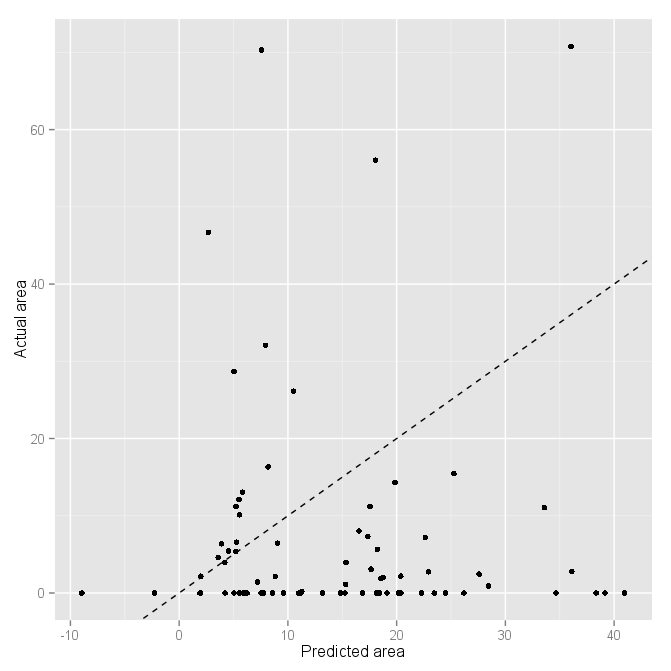
\includegraphics[width=0.4\textwidth]{figures/firenaivepredict.png}
  \caption{Raw data regression---predicted area versus actual area. Dotted line
  is the ideal case of perfect prediction}
\end{figure}

Clearly, our current model is not particularly accurate. In fact, the $R^2$
value for this run evaluates to a mere 0.0001555681. However, it will serve
well as a benchmark for testing the predictive abilities of other models
relative to this one. We now explore some possible transformations and/or
restrictions on the data set in an attempt to improve our predictions.

\subsection{Which data matters?}

We approach the task of narrowing our data range always with our goal in mind:
we are attempting to find the \emph{mean} area given knowledge of a set of
variables. Thus, it would make sense to remove the points which skew the mean
considerably.

The idea we used to break it down involved attempting to find a segment of data
where we have a relatively uniform amount of information for each range of
area. The easiest visual way we could determine this is by trimming down
outliers and showing the distribution of the area until it looks moderately
close to uniform. The difference between the distribution of area in the
original data and our trimmed data is shown in Figures 2 and 3.

\begin{figure}[htb]
  \begin{minipage}[b]{0.45\linewidth}
  \centering
  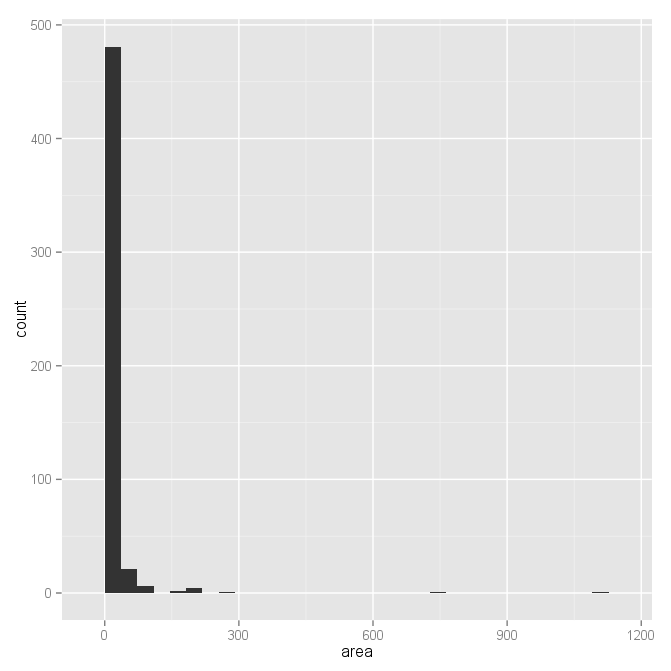
\includegraphics[width=\textwidth]{figures/badhist.png}
  \caption{Distribution of area with raw data}
\end{minipage}
\hspace{0.5cm}
  \begin{minipage}[b]{0.45\linewidth}
  \centering
  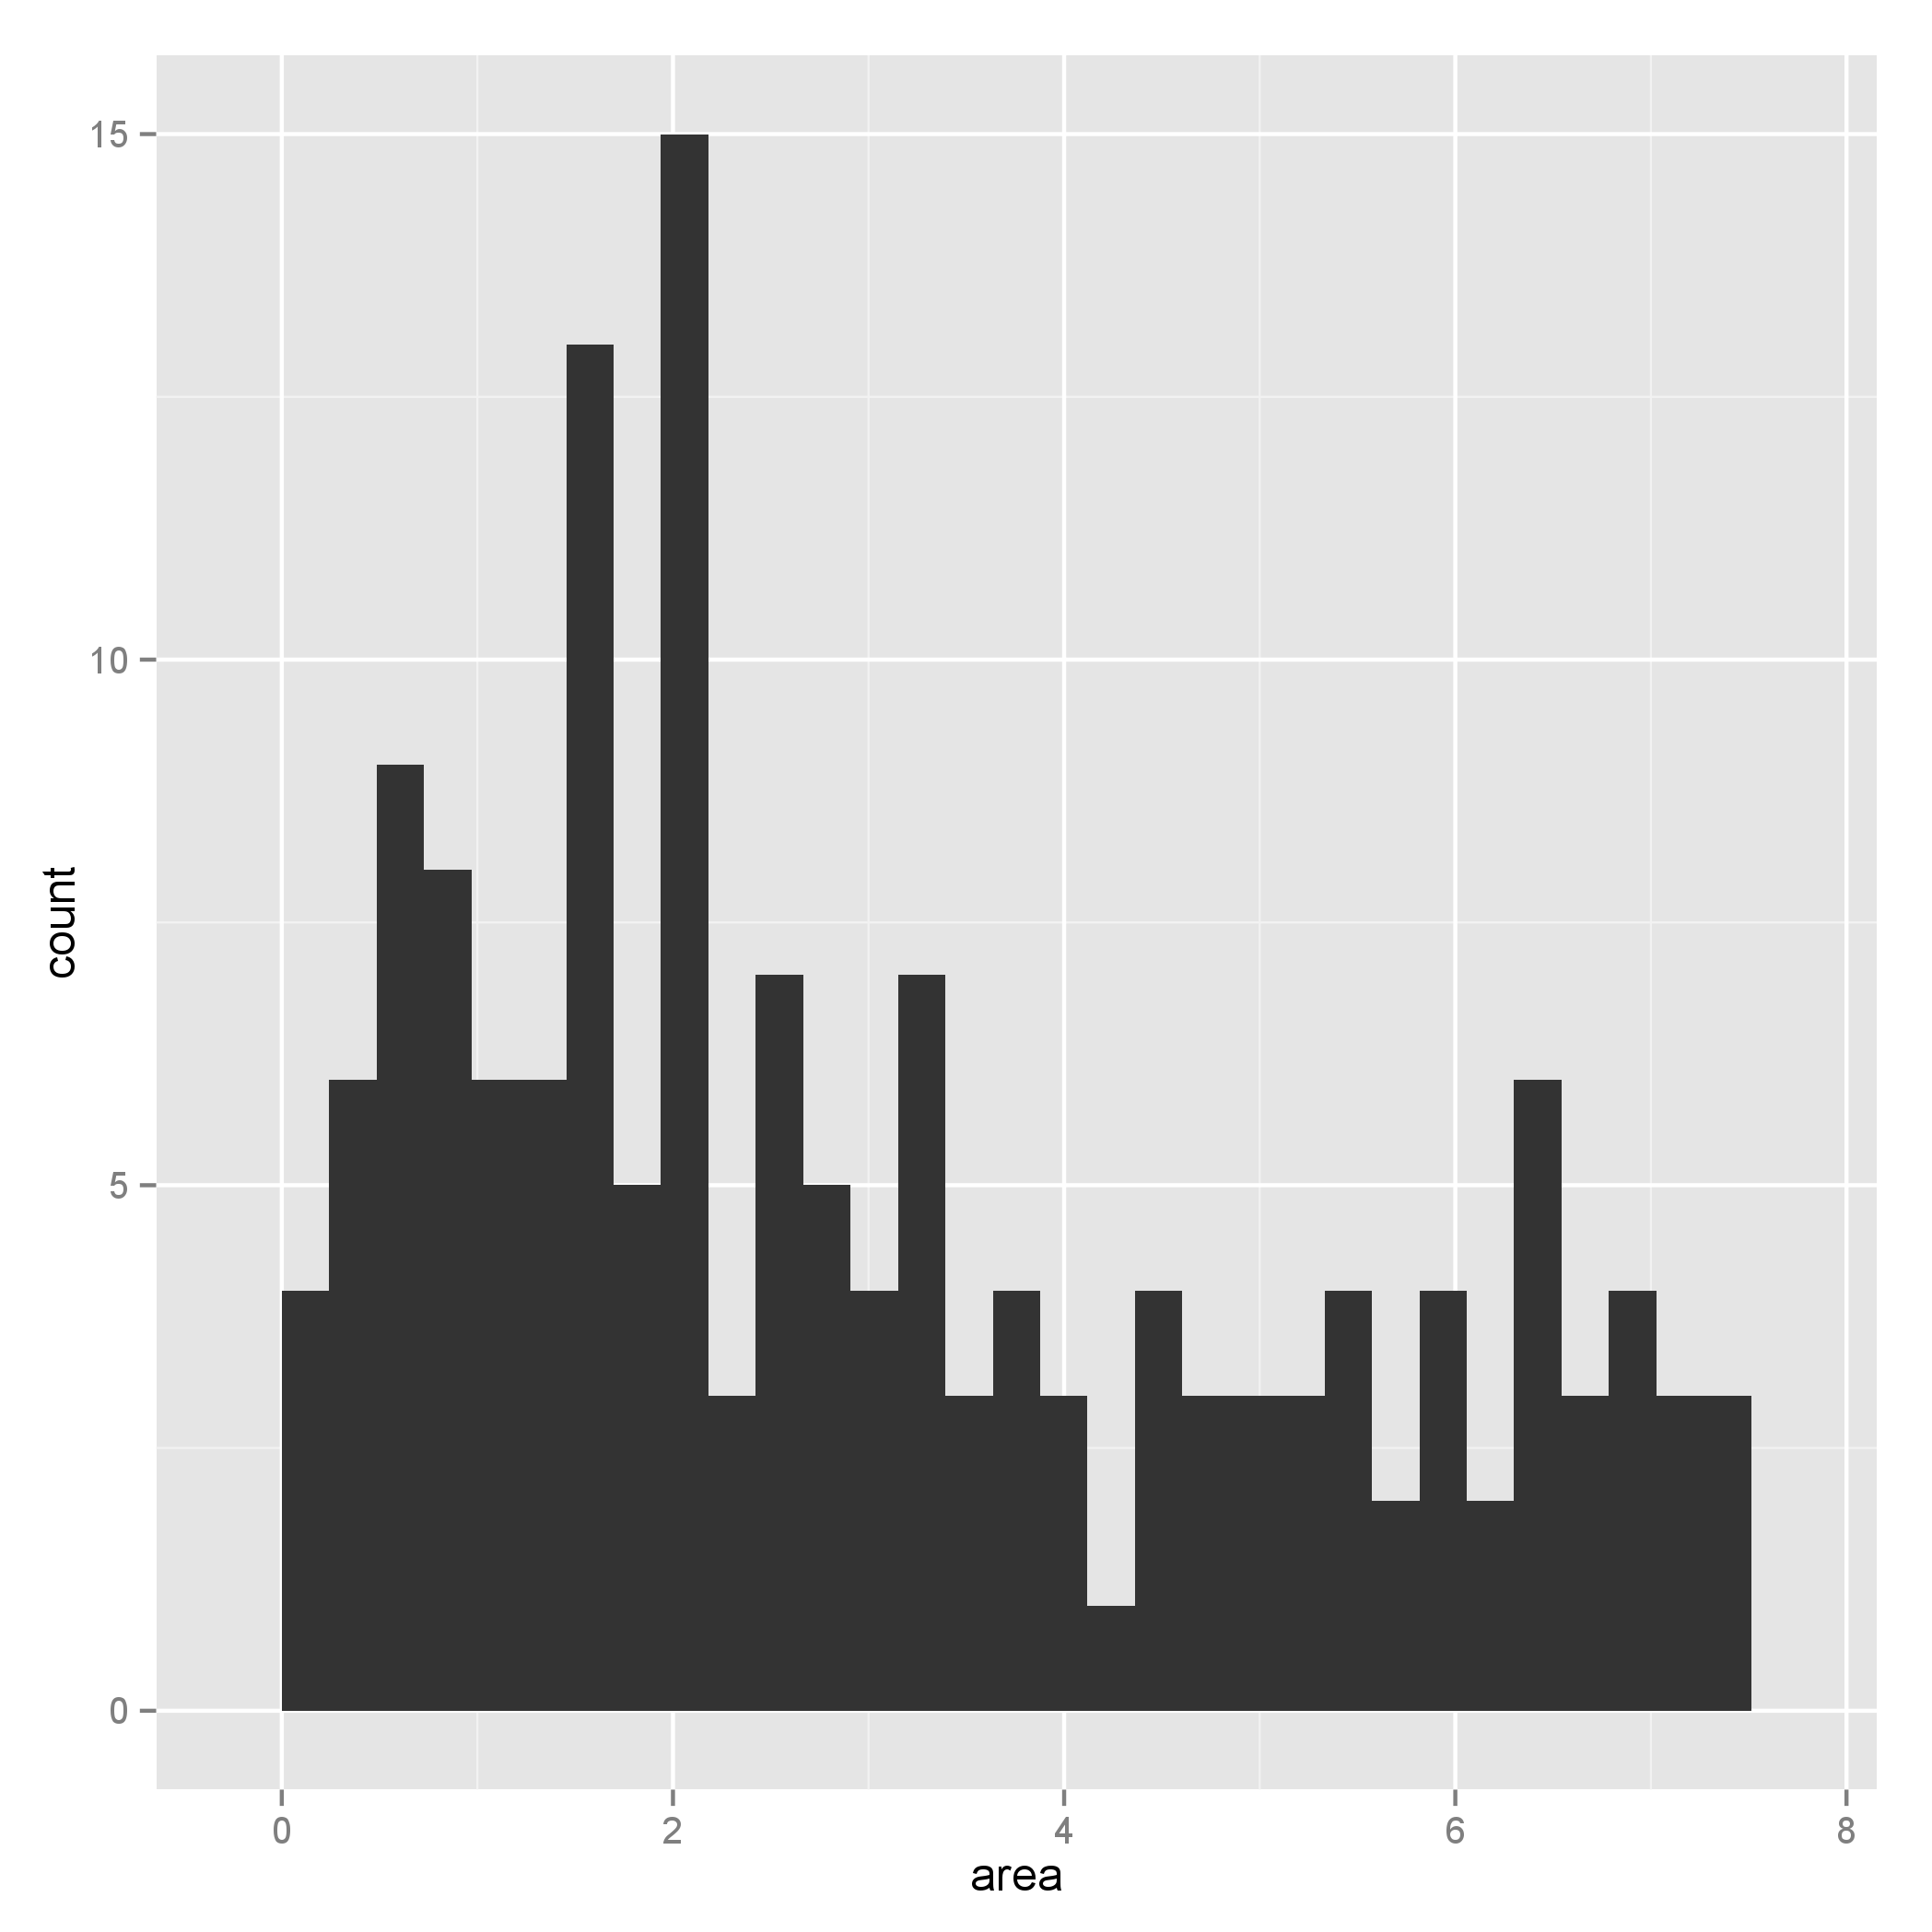
\includegraphics[width=\textwidth]{figures/goodhist.png}
  \caption{Distribution of area with trimmed data}
\end{minipage}
\end{figure}

Initially, doing variations and correlations between predictor variables and the response
variable resulted in abnormally low values. This led us to consider what the forest looked like.
We did this by creating a \verb+frequencyGrid+ and \verb+areaGrid+ that corresponds to each
of X,Y coordinates that exist. The data shown was below:

\begin{verbatim}
> frequencyGrid(data)
      [,1] [,2] [,3] [,4] [,5] [,6] [,7] [,8] [,9]
 [1,]    0    0    0    0    0    0    0    0    0
 [2,]   19   25    0    0    0    0    0    0    0
 [3,]   10    1    1   22    0   25    2    3    0
 [4,]   15   27   43   36   23    9   45    1    4
 [5,]    4   20    7   25    3   49   11    4    2
 [6,]    0    0    4    8    4    3    2   52    1
 [7,]    0    0    0    0    0    0    0    0    0
 [8,]    0    0    0    0    0    0    0    1    0
 [9,]    0    0    0    0    0    0    0    0    6

> areaGrid(data)
          [,1]    [,2]      [,3]      [,4]     [,5]      [,6]      [,7]      [,8]      [,9]
 [1,]      NaN     NaN       NaN       NaN      NaN       NaN       NaN       NaN       NaN
 [2,] 11.57579 18.5060       NaN       NaN      NaN       NaN       NaN       NaN       NaN
 [3,] 15.71400  0.0000 6.5800000  7.858182      NaN  7.711200 13.675000   8.77000       NaN
 [4,] 10.01867  5.3100 2.9383721 11.039722 3.206522 16.052222 10.541556  12.18000   46.4025
 [5,] 28.86750  4.6315 0.3114286 11.480400 0.000000 28.245918  7.035455   0.73250    4.0800
 [6,]      NaN     NaN 0.0000000 10.966250 4.405000  2.863333 43.225000  24.33269   42.8700
 [7,]      NaN     NaN       NaN       NaN      NaN       NaN       NaN       NaN       NaN
 [8,]      NaN     NaN       NaN       NaN      NaN       NaN       NaN 185.76000       NaN
 [9,]      NaN     NaN       NaN       NaN      NaN       NaN       NaN       NaN    0.7450
\end{verbatim}

\verb+frequencyGrid+ and \verb+areaGrid+ reveal several trends about the forest:

\begin{enumerate}
	\item $\approx 44\%$ of the forest locations never had a fire
	\item Locations with many fires usually have small mean areas
	\item Locations with few fires usually have large mean areas
\end{enumerate}

These trends suggested that certain parts of the data set were irrelevant to our prediction of
fire area. In order to predict fire size in the places that actually had fires, we decided to
ignore data that had particular X,Y coordinates with a mean area of NaN or frequency of 0.

\subsection{Predictor Selection 1}

For the second predictor set we decided to use the attributes that are part of the Fire Weather Index (FWI) such as FFMC, DMC, DC and ISI. 
Before we eliminated part of the data these values did now have a good $R^{2}$ value compared to the other meteorological data such as temperature, wind, humidity and rain. 
However, once we eliminated the data the attributes that are part of FWI gave us a far better $R^{2}$ value than the other meteorological variables. 
Using forward step-wise we started with FWI attributes, then we tested out different interaction terms between FWI attributes and found that $DMC \times FMC$  and $DC \times ISI$ greatly increased the $R^{2}$ of our regression.The only non FWI attribute we decided to go with was month because we saw a strong correlation between the months and the area.

\begin{align*}
  \widehat{m}_{area;FFMC,ISI,DC,month,DMC}(t) = &-23.1151201 - 0.2744283 \cdot t_1 + 0.3185786 \cdot t_2 \\
  &+ 0.0122545 \cdot t_3 + 2.5926093 \cdot t_4 \\
  &- 0.2495317 \cdot t_5 - 0.0006686 \cdot t_2 \cdot t_3 + 0.0027410 \cdot t_1 \cdot t_5 	   
\end{align*}
which is obtained from the output of \verb=lm=.

\begin{verbatim}
              		Estimate Std. Error t value Pr(>|t|)    
		(Intercept) 23.1151201  9.0213988   2.562 0.011419 *  
		FFMC        -0.2744283  0.1118159  -2.454 0.015301 *  
		ISI          0.3185786  0.1871206   1.703 0.090799 .  
		DC           0.0122545  0.0035439   3.458 0.000715 ***
		month        2.5926093  0.8779764   2.953 0.003673 ** 
		DMC         -0.2495317  0.1012981  -2.463 0.014935 *  
		ISI:DC      -0.0006686  0.0002937  -2.277 0.024264 *  
		FFMC:DMC     0.0027410  0.0011059   2.479 0.014335 *
\end{verbatim}

With this regression model we got an adjusted $R^{2}$ value of 0.09632 which was by far the best value we got at the time. Yet, this is still not a very good model for predicting the mean area of the fire. So then we decided to try another method of finding a good predictor set by using the backwards step-wise approach.

\subsection{Predictor Selection 2}
Backwards step-wise approach

\subsection{Final predictor set}

After testing various predictor selection methods, we came up with the following predictor set:
\begin{itemize}
	\item FFMC
	\item ISI
	\item DMC
	\item Month
	\item DC
	\item DC:ISI
	\item DMC:FFMC
\end{itemize}

\subsection{Cross validation}

to be filled...

%--------------------

\section{Parkinson's disease}

The dataset was created by Max Little of the University of Oxford, in collaboration with the
National Centre for Voice and Speech, Denver, Colorado, who recorded the speech signals. The
main aim of the data is to discriminate healthy people from those with PD, according to
"status" column which is set to 0 for healthy and 1 for PD. Our goal with this data is to
try to monitor patients with Parkinson's disease remotely, by simply analyzing their voices
on the phone.

\subsection{Possible Predictors}
MDVP.Fo.Hz.
\begin{verbatim}
                       Estimate Std. Error z value Pr(>|z|)    
(Intercept)            4.706084   0.775185   6.071 1.27e-09 ***
parkinson$MDVP.Fo.Hz. -0.022051   0.004446  -4.960 7.05e-07 ***
\end{verbatim}

We then found the mean value of MDVP.Fo.Hz. if the status was zero and got 181.9378 then we found the mean value if the status was one which was 145.1808. After we got these values we used the logistic equation and plugged the intercept value, the $\hat{\beta}$ and first the mean of MDVP.Fo.Hz to get a value of 0.6668947 which is not a good value for status 0 since we need it to be $\leq$ 0.5. We did the same thing but now using the mean of MDVP.Fo.Hz with status one and got a value of 0.8182747 which is higher than 0.5 but since the value that we got for status zero was bad we decided not to use this as one of our predictors.

We repeated these steps for the other variables and came up with the following data:

\begin{tabular}{l|c|c|c|c|c|c}
name & intercept & value & mean0 & mean1 & logit0 & logit1 \\
\hline
MDVP.Fhi.Hz. & 1.871388 & -0.003694 & 223.6368 & 188.4415 & 0.6668947 & 0.8182747 \\
\hline
MDVP.Flo.Hz. & 3.476248 & -0.019075 & 145.2073 & 106.8936 & 0.6696094 & 0.8080288 \\
\hline
MDVP.Jitter.Abs. & -1.0556 & 66665.3255 & 2.3375e-05 & 5.068027e-05 & 0.6230941 & 0.9107654 \\
\hline
spread1 & 15.8608 & 2.3966 & -6.759264 & -5.33342 & 0.416196 & 0.9560066 \\
\hline
spread2 & -2.4283 & 17.5354 & 0.160292 & 0.2481327 & 0.5944722 & 0.9996633 \\
\hline
PPE & -4.2214 & 32.2906 & 0.1230171 & 0.2338282 & 0.438044 & 0.9654122 \\
\hline
NHR & 0.4717 & 39.8604 & 0.01148271 & 0.02921095 & 0.7169546 & 0.8369981 \\
\hline
MDVP.Shimmer.dB & -1.497 & 12.353 & 0.1629583 & 0.3212041 & 0.6262175 & 0.9220717 \\
\hline
HNR & 7.0326 & -0.2576 & 24.67875 & 20.97405 & 0.662701 & 0.8361264 \\
\hline
RPDE & -2.4316 & 7.4058 & 0.4425519 & 0.5168159 & 0.699696 & 0.8015222 \\
\hline
DFA & -6.151 & 10.233 & 0.6957156 & 0.7254079 & 0.7247721 & 0.7811019 \\
\hline
\end{tabular}

Looking through these values we can see that spread 1 and PPE are the only ones that satisfy the condition in which we want logit of status zero to be $\leq$ 0.5 and logit of status 1 to be $<$ 0.5. This led us to starting to figure out the predictor set by first including PPE and spread 1.

\subsection{Predictor Selection 1}

We used the following:

\begin{equation}
\label{logit2}
m_{Y;X}(t) = P(Y = 1 | X = t) = \frac{1}{1+e^{-(\beta_0+\beta_1
t_1+...+\beta_r t_r)}}
\end{equation}

\begin{tabular}{l|c|c|r}
predictor & class 0 & class 1 & Comments \\
\hline
spread1 & 0.4 & 0.9 & Good! \\
PPE & 0.4 & 0.9 & Good! \\
\end{tabular}

\subsection{Predictor Selection 2}

\subsection{Final predictor set}

After testing various predictor selection methods, we came up with the following predictor set:
\begin{itemize}
	\item spread1
	\item PPE
\end{itemize}

\subsection{Cross validation}

to be filled...

%--------------------

\section{Beyond ECS 132}

Professor Devanbu's paper, "Clones: What is that smell?" assesses the validity of the "stink"
that surrounds clones.  This reputation stems from the long standing belief that clone's require
more project maintenance, as well as their tendency to create code bloat. One of the major
problems that people face with software life cycles is maintenance costs, which can require
around 80\% of the total cost. As a result, Devanbu and others have invested time in research
to minimize maintenance costs. One of the simplest ways to lower these costs involves
reducing defects in code. Three tests were structured to analyze the relationship between
clones and bugs. The first test determines the bug rate of cloned code; the second test
compares the bug rate in cloned code to that of regular code; and the last test checks
if prolific clone groups are buggier than the non-prolific clone groups. The results and
conclusions of each test were formulated using statistical computation and analysis.

The first test was an attempt to discover to what extent cloned code contributed to bugs.
The graph plots the cumulative bug convergence on the Y-axis against the clone ratio on the
X-axis. According the vertical line, which represents the average clone ratio across all
snapshots, both of the projects had that about 80\% of bugs have a lower clone ratio than
the overall project clone ratio. The test shows that in each case the bugs contained little
cloned code.

The second test finds whether clones occur more often in buggy code than elsewhere. A box
and whisker plot simply illustrates for all four projects that buggy code had a lower clone
ratio. This provides strong evidence that clones are not a large contributor of bugs. To
further support this claim, a second table displays the adjusted $p$ values in which a Wilcoxon
paired test is used as the null hypothesis and the alternative hypothesis is set to "snapshot
clone ratio $>$ bug clone ratio". Since the $p$ values shown are between 0.01 and 0.05, this
provides moderate evidence against the null hypothesis in favor of the alternative hypothesis.
In each of the four projects, clones were not a major source of bugs. This suggests that clones
are less buggy than regular code.

The third test assesses whether prolific clone groups are buggier than non-prolific clone groups.
This was accomplished by finding the defect density in prolific clone groups and comparing it to
those found in non-prolific clone groups. Figure 2 utilizes the resulting data in a box and whisker
plot. The graph shows that in each case the bug density in prolific clone groups is lower than that
of the non-prolific clone group. In addition, table three utilizes a Wilcoxon test with the alternative
hypothesis set to "defect density in non-prolific groups $>$ defect density of prolific group" provides
$p$ values that are below 0.5. These $p$ values reject the null hypothesis in favor of the alternative,
providing evidence in that more prolific clone groups are less buggy than non-prolific clone groups.

In each of the three tests, the clones were falsely attributed to a bad trait. Since the four
projects used were medium to large open source projects, this data should be applicable
in most situations. One area of contention over these results is how cloned code is identified.
To address this issue, the tests were applied to two separate data sets. The first data set
uses a conservative clone detector, while the second employs a more liberal one. Both detectors
require 50 tokens in length to consider a code segment to be cloned, but the liberal detector
allows for 1\% less similarity than that of the conservative detector. Since analyzing both
data sets led to the same conclusion, the difference in detection methods is negligible. Ultimately,
the evidence from each test shows that clones may have unfairly garnered a bad reputation.

\pagebreak

\appendix
\section{Code}
\subsection{Problem 1}
\lstinputlisting[caption=Analysis for Forest Fire Data Set]{p1.R}
\subsection{Problem 2}
\lstinputlisting[caption=Analysis for Parkinson's Data Set]{p2.R}

\section{Who did what}
\begin{itemize}
	\item Aaron - implemented R functions for Problem 1 and 2 and did initial analysis
	\item Anatoly - assisted Aaron in development of Problem 1 and 2 code; used code to generate plots
	\item Justin - used Devanbu's article to finish Problem 3
	\item Samuel - wrote R to do initial analysis, copy-edited Problem 3 and did write-up for Problem 1 and 2
\end{itemize}

\end{document}             % End of document.
